\documentclass[12pt]{article}

\usepackage[a4paper,top=3cm,bottom=2cm,left=2cm,right=2cm,marginparwidth=1.2cm]{geometry}
\usepackage{fancyhdr}
\usepackage{graphicx}
\usepackage{float}
\usepackage{xcolor}
\usepackage{pgfplots}
\usepackage{caption}
\usepackage{mdframed}
\usepgfplotslibrary{fillbetween}
\pgfplotsset{compat=1.18}
\graphicspath{{./}}
\usepackage{float}

\author{Eden Li}
\title{STAT110/115 Tutoring Materials – ANOVA}
\date{}

\begin{document}
\pagestyle{fancy}
\lhead{STAT110/115 Tutoring Materials}
\rhead{ANOVA}

\begin{itemize}
\item \textbf{ANOVA}: Abbreviation of \textbf{Analysis of Variance}.
\item \textbf{Methods for comparing means} of continuous responses between multiple groups.
\item \textbf{F-ratio}: Signal/noise
\begin{figure}[H]
    \centering
    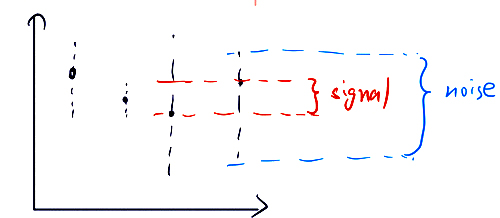
\includegraphics[width=0.4\textwidth]{anova.jpg}
\end{figure}
\item \textbf{Reasons why using "2+2+2=3" is undesirable}:
    \begin{itemize}
    \item It's more work than we need to do. Three tests may not seem too bad, but to compare 10 groups we would have to do 45 different pairwise t-tests.
    \item It can lead to lots of false positive results. Every test has the potential to incorrectly reject H0; i.e. falsely identify a difference between a pair of groups. If we do lots of tests then we risk generating lots of false positives.
    \end{itemize}
\item \textbf{ANOVA model}: 
$$Y_{ij}=\mu_i+e_{ij}$$
$\mu_i$ is the true mean response for the ith group at the population level. $e_{ij}$ is the error term for the jth response in the ith group. The error terms are assumed to be independent and to follow a N(0, $\sigma^2$) with constant variance. The number of different groups is denoted K, and the number of responses in the ith group is denoted $n_i$.
\item \textbf{Est. mean for ANOVA}: The "." = est. Value.
$$\hat{\mu}_i = \bar{y}_i.$$
\item \textbf{Sample mean for the ith group:}
$$\bar{y}_i.=\frac{1}{n_i}\sum_{j=1}^{n}y_{ij}$$
\item \textbf{Formula for residual sum of squares in ANOVA} (no need to memorise):
$$RSS=\sum_{i=1}^{K}\sum_{j=1}^{n_i}(y_{ij}-\hat{\mu}_i)^2=\sum_{i=1}^{K}\sum_{j=1}^{n_i}(y_{ij}-\bar{y}_i.)^2$$
\item \textbf{Total sum of squares in ANOVA} (no need to memorise):
$$TSS=\sum_{i=1}^{K}\sum_{j=1}^{n_i}(y_{ij}-\bar{y}..)^2$$
\item \textbf{$y..$} is the sample mean overall the data.
\item \textbf{Formula for GSS in ANOVA} (no need to memorise): 
$$GSS = TSS - RSS$$ 
$$GSS = \sum_{i=1}^{k}n_i(\bar{y}_i.-\bar{y}..)^2$$
GSS can be interpreted as a measure of the variation that is explained by differences between groups.
\item \textbf{Setting up the hypotheses to test ANOVA:}

As usual, the null hypothesis will be the 'no difference' hypothesis:
$$H_0: \mu_1=\mu_2=...=\mu_K$$
The alternative is simply an expression that the null is incorrect:

\centerline {$H_A:\mu_1, \mu_2, ..., \mu_K$ not all equal.}

\item \textbf{Equation for F statistic:}
$$F = \frac{GSS/(K-1)}{RSS/(n-K)}$$
\item \textbf{GMS}: GSS/(K - 1) is the group mean square.
\item \textbf{RMS}: RSS/(n - K) is the residual mean square.
\item \textbf{What situations would let $H_0$ fail}: Large differences between group means. Relatively large value of GSS. A large value of F.
\item \textbf{ANOVA table:}
\begin{table}[h]
\centering
\begin{tabular}{lccc}
\hline
Source & SS & DF & MS \\ \hline
Groups & GSS & $K - 1$ & $\frac{GSS}{K - 1}$ \\
Residuals & RSS & $n - K$ & $\frac{RSS}{n - K}$ \\ \hline
Total & TSS & $n - 1$ \\ \hline
\end{tabular}
\end{table}
\item \textbf{P-value is right censored}.
\item \textbf{Blocking variable}: A second treatment variable that when included in ANOVA analysis will have the effect of reducing the SSE term (noise).
\end{itemize}

\end{document}
